\normalfalse \difficiletrue \tdifficilefalse
\correctiontrue

%\UPSTIidClasse{11} % 11 sup, 12 spé
%\newcommand{\UPSTIidClasse}{12}

\exer{Mouvement RR -- RSG  $\star\star$ \label{B2:13:46}}
\setcounter{question}{0}\marginnote{\UPSTIcompetence{B2-13}}
\index{Compétence B2-13}
\index{Mécanisme à 2 rotations et RSG}
\index{Segway}
\ifcorrection
\else
\marginnote{\textbf{Pas de corrigé pour cet exercice.}}
\fi

\ifprof
\else
Soit le mécanisme suivant. On a $\vect{IA}=R\vect{j_0}$ et $\vect{AB}=L\vect{i_2}$. De plus $R=\SI{15}{mm}$. On fait l'hypothèse de roulement sans glissement au point $I$.
\begin{center}
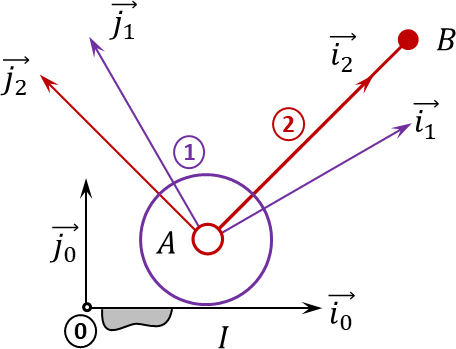
\includegraphics[width=.8\linewidth]{46_RR_RSG_01}
\end{center}
\fi


\question{Déterminer $\vectv{B}{2}{0}$.}
\ifprof
En utilisant la décomposition du vecteur vitesse : 
$\vectv{B}{2}{0} = \vectv{B}{2}{1} +  \vectv{B}{1}{0}$.

\begin{itemize}
\item \textbf{Calcul de $ \vectv{B}{2}{1}$ :}  $\babarv{B}{A}{2}{1}$. 2 et 1 étant en pivot d'axe $\axe{A}{k_0}$, on a $\vectv{B}{2}{1}=\vect{0}-L\vi{2}\wedge \varphip(t)\vk{0}$
$=L\varphip(t)\vj{2}$.
\item \textbf{Calcul de $ \vectv{B}{1}{0}$ :}  $\babarv{B}{I}{1}{0}$ 
$=\vect{0}-L\vi{2}\wedge \varphip(t)\vk{0}$. En utilisant l'hypothèse de roulement sans glissement : $ \vectv{B}{1}{0}$  $=\left(-L\vi{2}-R\vj{0}\right)\wedge \thetap(t)\vk{0}$  $=\thetap(t)\left(L\vj{2}-R\vi{0}\right)$.
\end{itemize}

Au final, $\vectv{B}{2}{0} = L\varphip(t)\vj{2} +\thetap(t)\left(L\vj{2}-R\vi{0}\right) $.


\else
\fi

\question{Donner le torseur cinématique $\torseurcin{V}{2}{0}$ au point $B$.}
\ifprof
 $\torseurcin{V}{2}{0} = \torseurl{\vecto{2}{0}=\left( \varphip(t)+\thetap(t) \right) \vk{0} }{ L\varphip(t)\vj{2} +\thetap(t)\left(L\vj{2}-R\vi{0}\right)}{B}$.
 

\else
\fi

\question{Déterminer $\vectg{B}{2}{0}$.}

\ifprof
$\vectg{B}{2}{0} = \deriv{\vectv{B}{2}{0}}{\rep{0}}$

$ = \deriv{L\varphip(t)\vj{2}}{\rep{0}} + \deriv{\thetap(t)\left(L\vj{2}-R\vi{0}\right)}{\rep{0}}$

$ = L\varphipp(t)\vj{2}-L\varphip(t)\left(\varphip(t)+\thetap(t) \right)\vi{2}  + \thetapp(t)\left(L\vj{2}-R\vi{0}\right) - L\thetap(t)\left(\varphip(t)+\thetap(t) \right)\vi{2}$.



\else
\fi


\ifprof
\else
\ifcolle
\else
\begin{solution}[A Vérifier...]
\begin{enumerate}
\item $\vectv{B}{2}{0} = L\varphip(t)\vj{2} +\thetap(t)\left(L\vj{2}-R\vi{0}\right) $.
\item  $\torseurcin{V}{2}{0} = \torseurl{\vecto{2}{0}=\left( \varphip(t)+\thetap(t) \right) \vk{0} }{ L\varphip(t)\vj{2} +\thetap(t)\left(L\vj{é}-R\vi{0}\right)}{B}$.
\item $\vectg{B}{2}{0} =  L\varphipp(t)\vj{2}-L\varphip(t)\left(\varphip(t)+\thetap(t) \right)\vi{2}  + \thetapp(t)\left(L\vj{2}-R\vi{0}\right) - L\thetap(t)\left(\varphip(t)+\thetap(t) \right)\vi{2}$.
\end{enumerate} 
\end{solution}
\fi

\marginnote{Corrigé  voir \ref{B2:13:46}.}

\fi